\documentclass{lecturefig}
\begin{document}
\newcommand{\V}[2][]{\tikz[remember picture,baseline]\node[anchor=base,draw,#1,minimum size=0,inner sep=2pt,
                       every V/.try]{\mathstrut\ttfamily #2};}

\def\x{\V[minimum width=0,fill=amber!60,name=x]{x}}
\def\y{\V[minimum width=0,fill=safegreen!40,name=y]{y}}
\def\z{\V[minimum width=0,fill=luhblue!40,name=z]{z}}

\begin{frame}[fragile]
  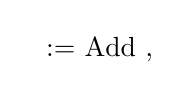
\begin{tikzpicture}[]
    \node{\x{} := Add \y{}, \z{}};
  \end{tikzpicture}
\end{frame}
\begin{frame}[fragile]
  \begin{tikzpicture}[remember picture]
    \node[draw,fill=badbee!40,minimum height=3\baselineskip,minimum width=4cm,
              alt=<-3>{}{text opacity=0}]
        (operation)
        {add \V[fill=white,name=r1]{r1}, \V[fill=white,name=r2]{r2}};


    \begin{visible}<2-3>
      \node[width as=r1,draw,fill=white,anchor=east,xshift=-1ex] at (operation.north) (l1) {\scriptsize load $\rightarrow$ r1};
      \node[width as=r2,draw,fill=white,anchor=west,xshift=1ex] at (operation.north) (l2) {\scriptsize load $\rightarrow$ r2};
      \node[width as=r2,draw,fill=white] at (operation.south) (s1) {\scriptsize r2 $\rightarrow$ store};
    \end{visible}

    \begin{pgfonlayer}{background}
    \begin{visible}<3->
      \node[above=-\pgflinewidth of operation,width as=operation,fill=luhgray!50,draw,align=center,
          alt=<3>{}{text opacity=0},
      ]
        (area-top) {\y{}\hspace{2.5cm}\z\\};

      \node[below=-\pgflinewidth of operation,width as=operation,fill=luhgray!50,draw,align=center,
            alt=<3>{}{text opacity=0},
      ]
      (area-bottom) {\mbox{}\\\hspace{2.5cm}\x};

      \begin{visible}<3>
        \draw[->] (y) to[out=0, in=90] ($(l1.north east)+(west:2ex)$);
        \draw[->] (z) to[out=180, in=90] ($(l2.north west)+(east:2ex)$);
        \draw[->] (s1) to[out=-90, in=180] (x);
      \end{visible}
    \end{visible}
  \end{pgfonlayer}

  \begin{visible}[my text/.style={
      align=left,
      font=\ttfamily,
      inner ysep=0
      }]<4-5>
    \node[above=0 of operation.north west,anchor=south west,my text] {
        \strut mov \alt<4>{\y}{8(\%ebp)}, \%eax\\
        \strut mov \alt<4>{\z}{-8(\%ebp)}, \%ebx
      };

      \node[at=(operation.west), anchor=west,my text] {
        \strut add \%eax, \%ebx
      };
      
      \node[below=0.1 of operation.south west,anchor=north west,my text] {
        mov \%ebx, \alt<4>{\x}{-4(\%ebp)}
      };

  \end{visible}

    


  \end{tikzpicture}
\end{frame}
\end{document}
